% 2003 年河南卷第 17 题：直角坐标系函数图象（解析答案图）
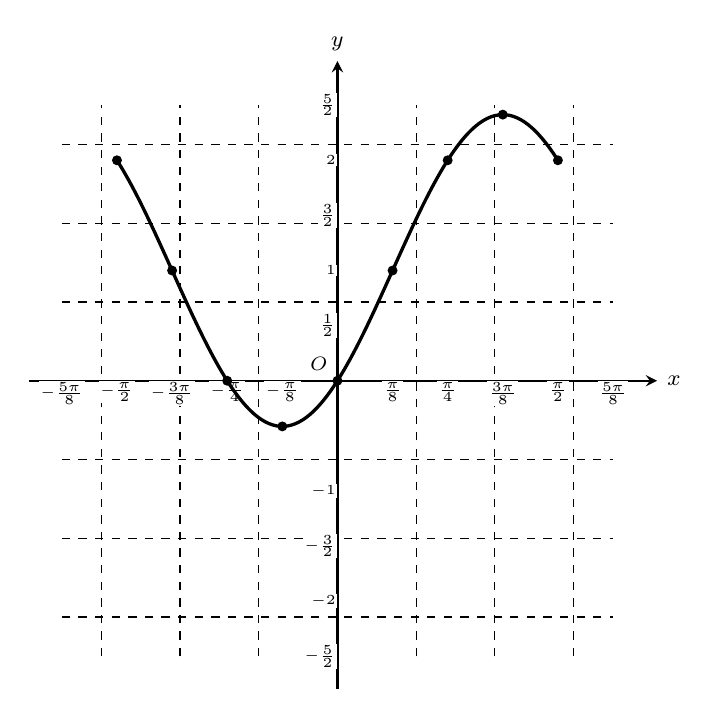
\begin{tikzpicture}[x=0.7cm,y=0.7cm,>=stealth]
  % Dashed grid
  \draw[dashed,thin] (-5,-5) grid (5,5);
  % Axes
  \draw[->,thick] (-5.6,0) -- (5.8,0) node[right] {\footnotesize $x$};
  \draw[->,thick] (0,-5.6) -- (0,5.8) node[above] {\footnotesize $y$};
  % Origin
  \node[above left] at (0,0) {\scriptsize $O$};
  
  % y-ticks and labels
  \node[left,fill=white,inner sep=0.5pt] at (0,1) {\tiny $\frac{1}{2}$};
  \node[left,fill=white,inner sep=0.5pt] at (0,2) {\tiny $1$};
  \node[left,fill=white,inner sep=0.5pt] at (0,3) {\tiny $\frac{3}{2}$};
  \node[left,fill=white,inner sep=0.5pt] at (0,4) {\tiny $2$};
  \node[left,fill=white,inner sep=0.5pt] at (0,5) {\tiny $\frac{5}{2}$};
  \node[left,fill=white,inner sep=0.5pt] at (0,-2) {\tiny $-1$};
  \node[left,fill=white,inner sep=0.5pt] at (0,-3) {\tiny $-\frac{3}{2}$};
  \node[left,fill=white,inner sep=0.5pt] at (0,-4) {\tiny $-2$};
  \node[left,fill=white,inner sep=0.5pt] at (0,-5) {\tiny $-\frac{5}{2}$};

  % x-ticks and labels
  \node[below,fill=white,inner sep=0.5pt] at (-5,0) {\tiny $-\frac{5\pi}{8}$};
  \node[below,fill=white,inner sep=0.5pt] at (-4,0) {\tiny $-\frac{\pi}{2}$};
  \node[below,fill=white,inner sep=0.5pt] at (-3,0) {\tiny $-\frac{3\pi}{8}$};
  \node[below,fill=white,inner sep=0.5pt] at (-2,0) {\tiny $-\frac{\pi}{4}$};
  \node[below,fill=white,inner sep=0.5pt] at (-1,0) {\tiny $-\frac{\pi}{8}$};
  \node[below,fill=white,inner sep=0.5pt] at (1,0) {\tiny $\frac{\pi}{8}$};
  \node[below,fill=white,inner sep=0.5pt] at (2,0) {\tiny $\frac{\pi}{4}$};
  \node[below,fill=white,inner sep=0.5pt] at (3,0) {\tiny $\frac{3\pi}{8}$};
  \node[below,fill=white,inner sep=0.5pt] at (4,0) {\tiny $\frac{\pi}{2}$};
  \node[below,fill=white,inner sep=0.5pt] at (5,0) {\tiny $\frac{5\pi}{8}$};

  % Plotted curve
  \draw[very thick,domain=-4:4,samples=120,smooth] plot (\x, {2 + 2*sqrt(2)*sin(45*\x - 45)});
  % Key points
  \foreach \coord in {(-4,4), (-3,2), (-2,0), (-1,{2-2*sqrt(2)}), (0,0), (1,2), (2,4), (3,{2+2*sqrt(2)}), (4,4)} {
    \fill \coord circle (1.8pt);
  }
\end{tikzpicture}
